\section{Phases d’approche avant l’atterrissage}

\subsection{Première phase d’approche : placement de l’UAV via localisation GNSS}

Pour rejoindre l’UGV afin de de réaliser le docking, le drone d’inspection doit dans un premier temps s’en approcher jusqu’à le survoler. Le drone doit alors rejoindre la position de l’UGV en mouvement à une certaine altitude donnée, comme s'il devait atteindre un “waypoint” mobile en connaissant sa position géographique.

\begin{figure}[H]
    \centering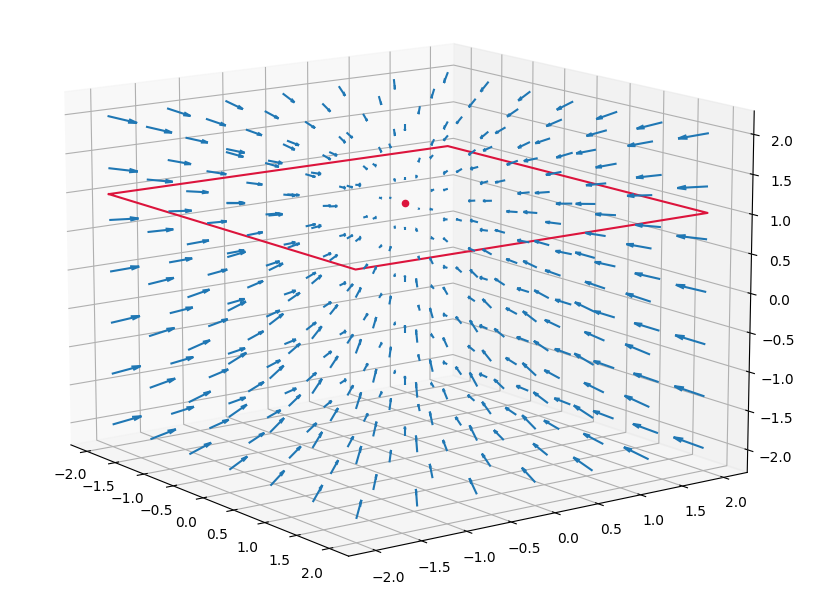
\includegraphics[width=0.5\textwidth]{images/phases_approche/potent_phase_1.png}
    \caption{Représentation du champ de potentiel lors de la phase d'approche via géolocalisation \cite{quiver}}
\end{figure}

La méthode que nous avons choisie est la suivante : en comparant les coordonnées GNSS des deux robots, on construit un champ de potentiel qui force l’UAV à rejoindre un point qui se situe juste au-dessus de l’UGV. Ce champ de potentiel vise à amener d’abord le drone sur un plan horizontal à altitude fixe au-dessus de la plateforme, puis de faire converger sa position sur l’axe central de la descente.
L'asservissement par coordonnées GNSS s’arrête dès que la plateforme munie de marqueurs ArUco est détectée par la caméra embarquée sur l’UAV. Il est alors possible de positionner le drone avec davantage de précision grâce aux outils de localisation dans l’espace de vision 3D.

\subsection{Seconde phase d’approche : descente dans un cône virtuel par vision 3D}

Une fois le drone positionné au-dessus de l’UGV, les marqueurs ArUco placés sur sa plateforme sont maintenant visibles par la caméra embarquée sur l’UAV. A l’aide d’outils de vision 3D disponibles avec les librairies OpenCV et ArUco, il est possible de détecter des marqueurs et de déterminer la position relative dans l’espace par rapport à la caméra du drone. Ainsi le drone est capable de se positionner avec une précision de l’ordre de 10 centimètres, afin d’entamer une descente progressive vers l’UGV.

\begin{figure}[H]
    \centering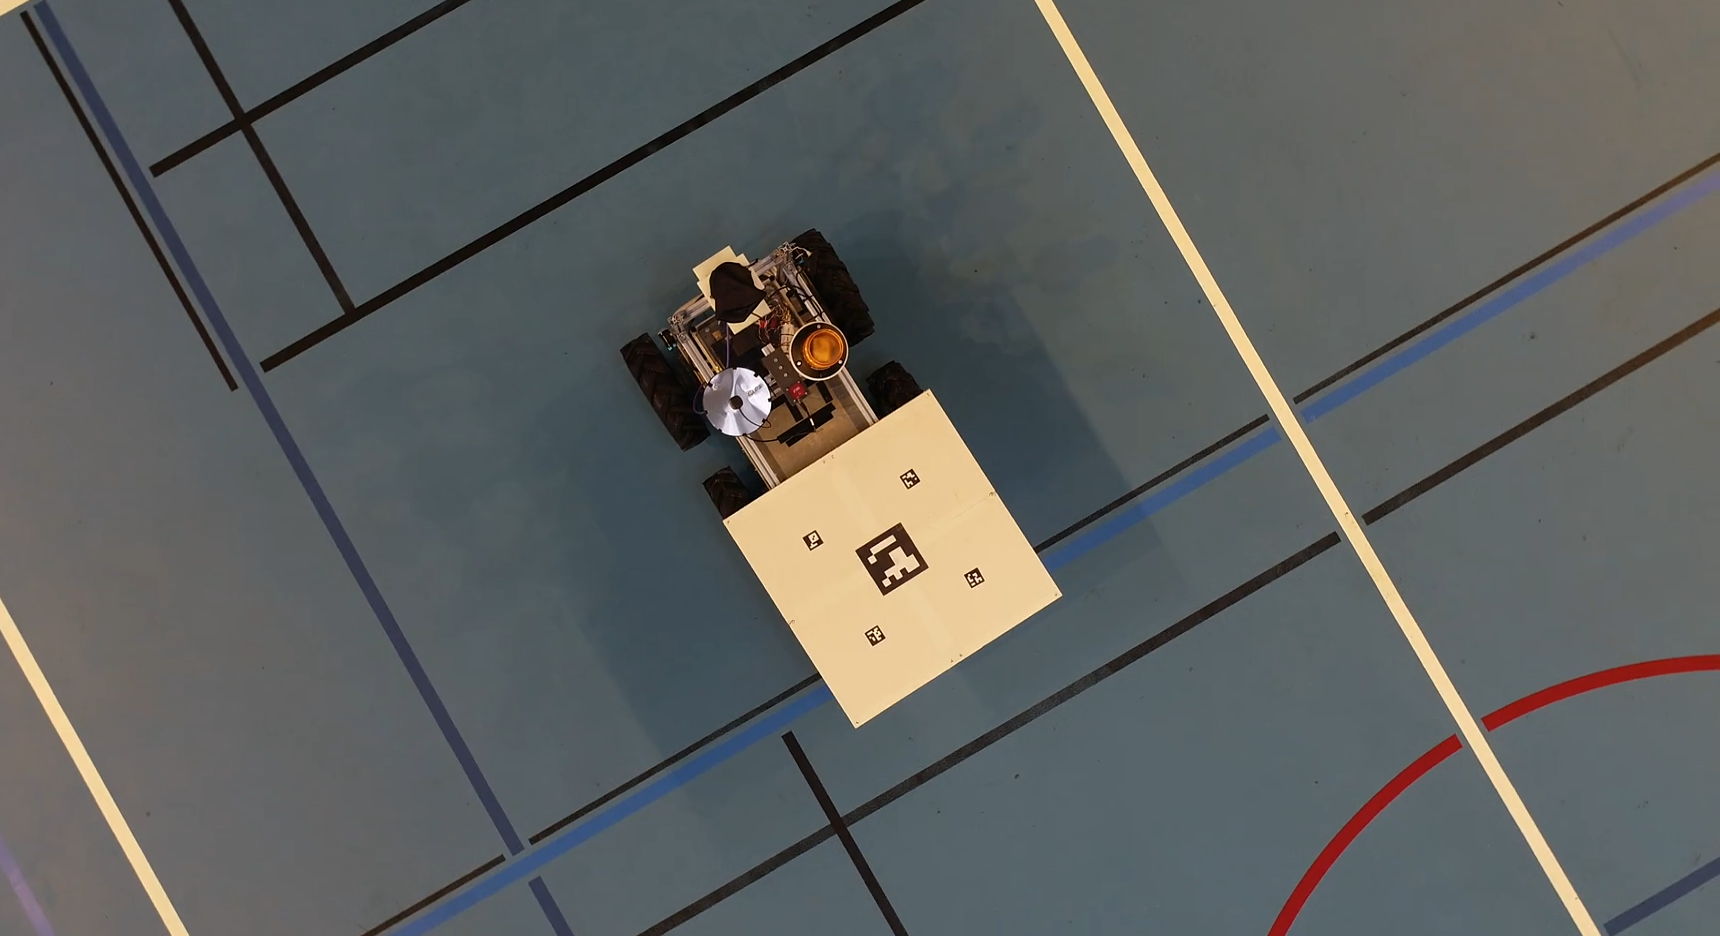
\includegraphics[width=0.5\textwidth]{images/phases_approche/ugv_upview.png}
    \caption{Vue sur l'UGV depuis la caméra du drone}
\end{figure}

La méthode que nous proposons suppose un cône virtuel dans lequel le drone à la manœuvre doit se trouver pour ne pas risquer de perdre de vue les marqueurs ArUco essentiels à sa propre localisation. Si l’UAV sort de ce cône virtuel, il a pour ordre de repasser dans la première ĥase d’approche, afin de la mettre en sécurité à altitude fixe, et de faire converger la position du drone au dessus de l’UGV. Afin de le maintenir proche de cet axe lors de la descente, l’UAV est guidé par un champ de potentiels dirigés vers le centre de la plateforme. Ce champ de potentiel vise d’abord à attirer le drone vers la droite de révolution du cylindre virtuel puis à le faire descendre sur l’UGV.

\begin{figure}[H]
    \centering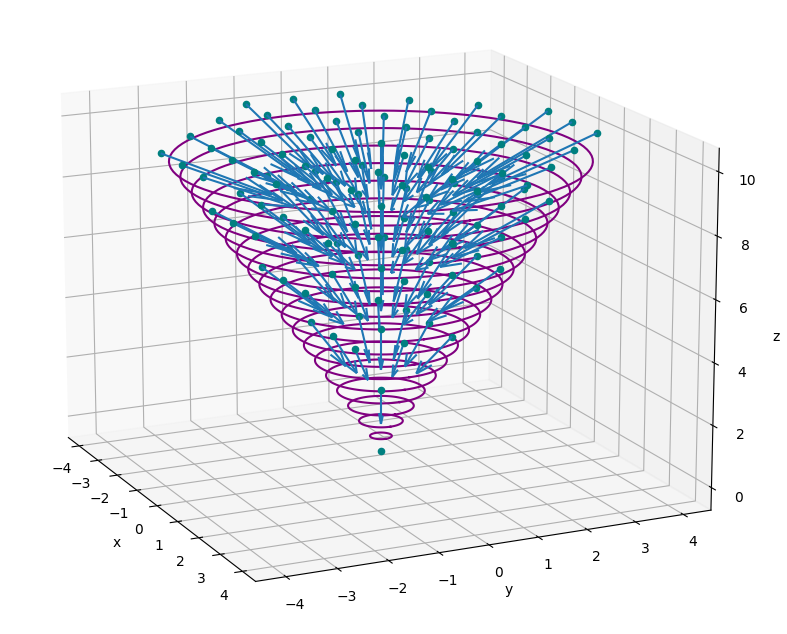
\includegraphics[width=0.5\textwidth]{images/phases_approche/potent_phase_2.png}
    \caption{Représentation du champ de potentiels lors de la phase de déscente dans le cône virtuel \cite{quiver}}
\end{figure}